%!tex program = lualatex
\documentclass{ctexart}
\usepackage{graphicx}
\usepackage[margin=2cm]{geometry}
\usepackage{amsmath}
\usepackage{amssymb}
\usepackage{tikz}
\usetikzlibrary{calc, patterns, intersections}
\pagestyle{empty}
\newcounter{xcord}
\newcounter{ycord}
\newcounter{total}
\ctexset{
	subsection/name = {第,题},
	subsection/number = {\thesubsection},
	section ={
		name = {第,部分}
	}
}
\renewcommand{\labelenumi}{\textbf{\ifnum\value{enumi}<10 0\fi\arabic{enumi})}}
\begin{document}
\section*{求阴影面积}
\begin{center}
	\begin{tikzpicture}
		\node(x){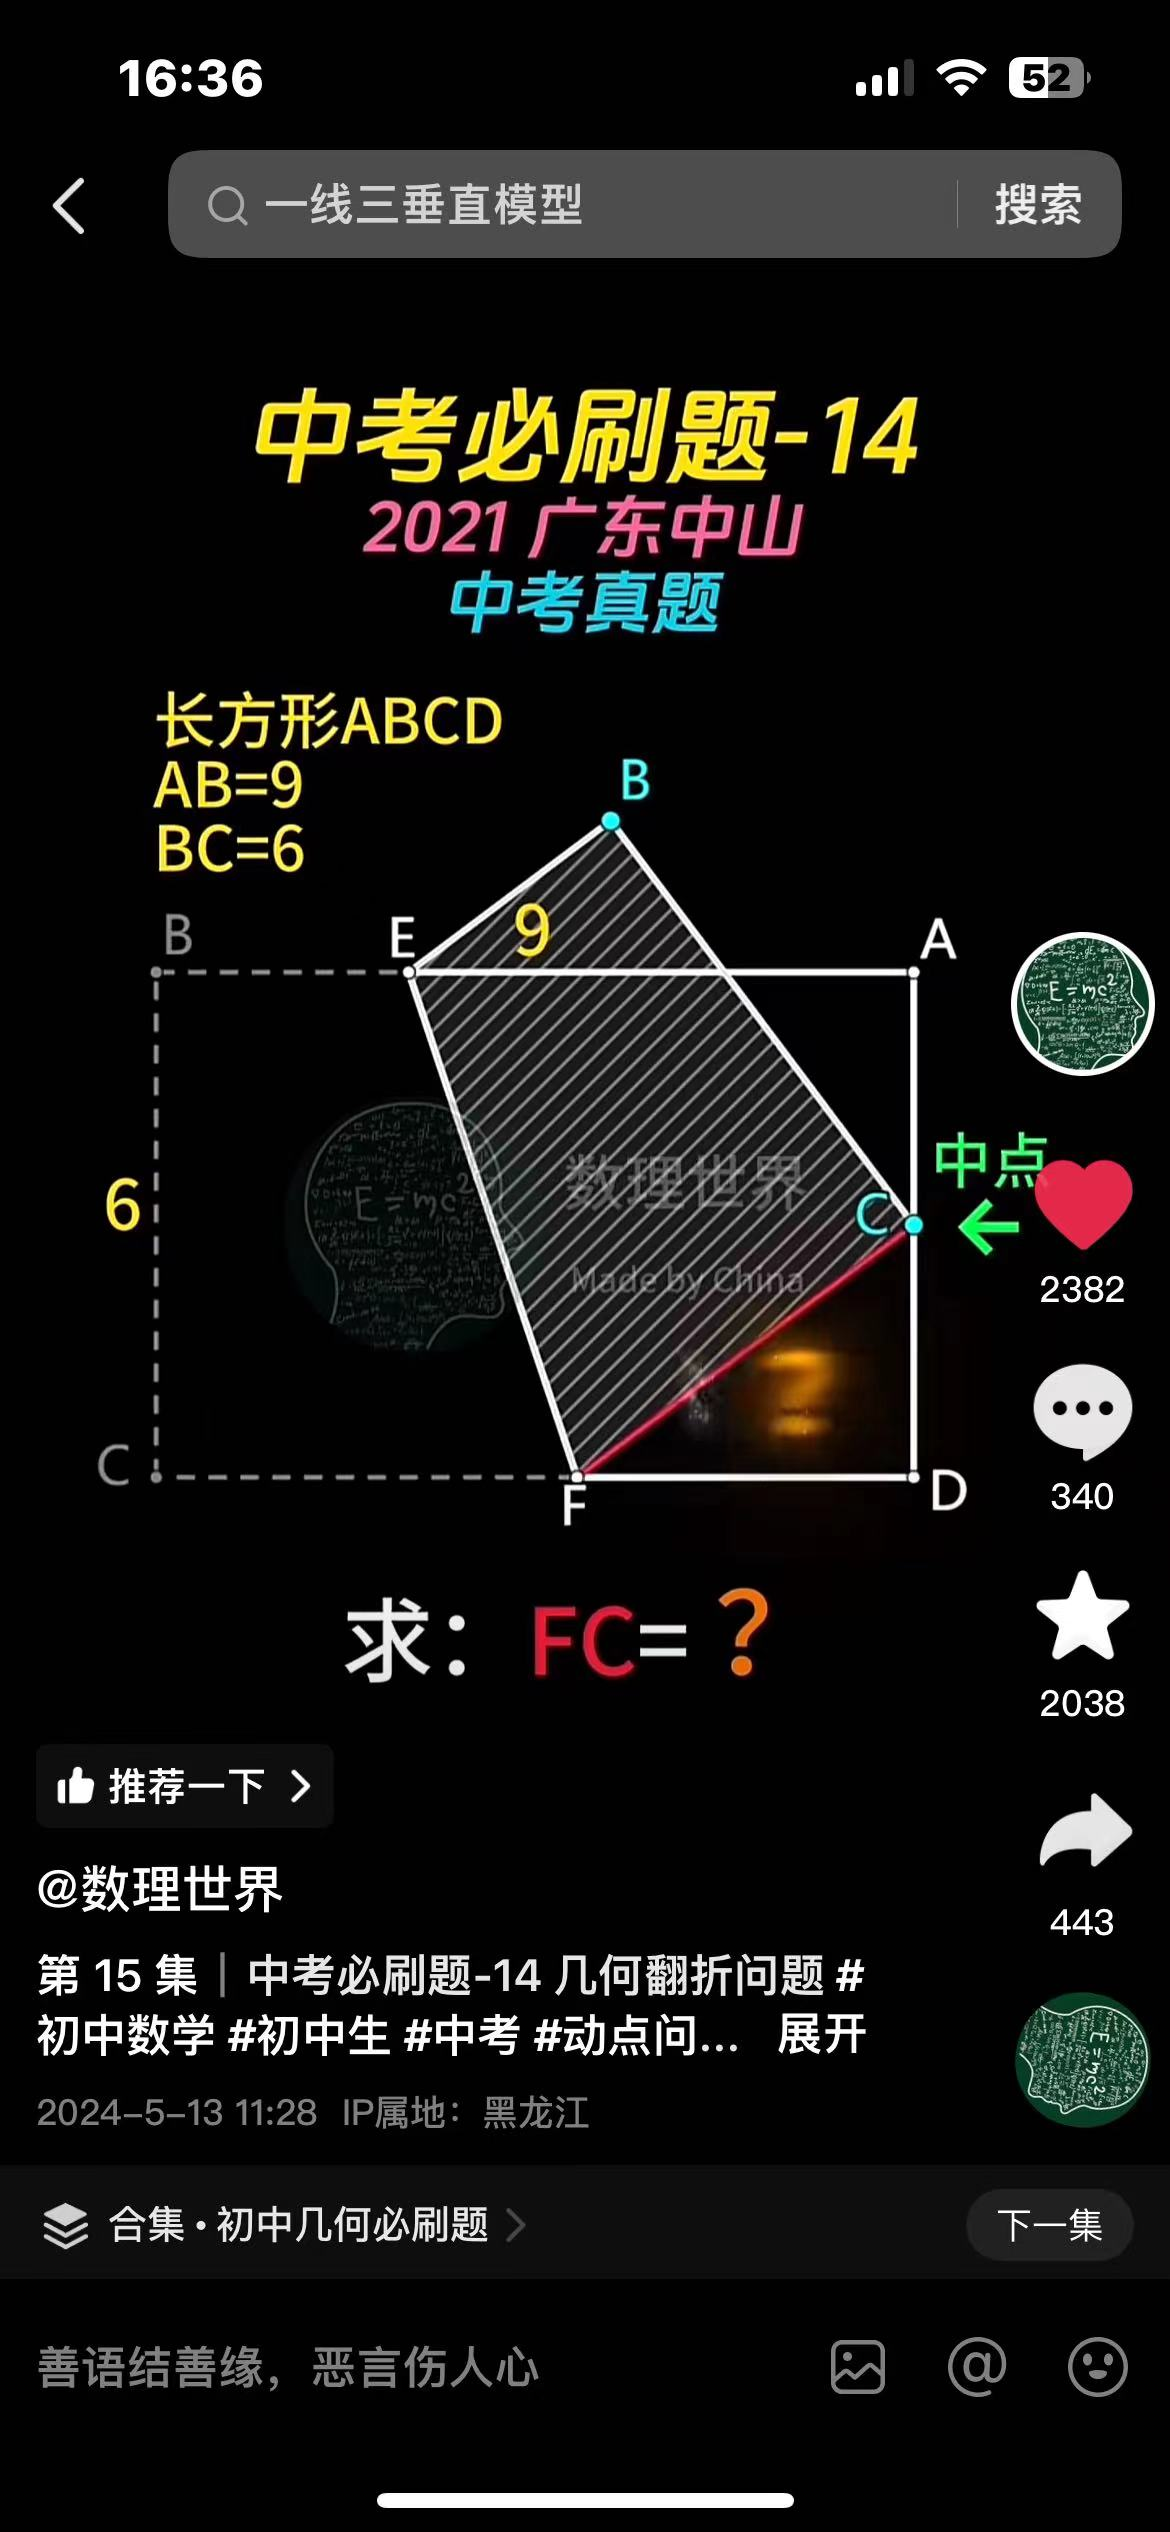
\includegraphics[scale=.1]{WechatIMG1.jpg}};
		\node at (x.center) [yshift=1.3cm, xshift=.8cm]{\color{red}\Large $G$};
	\end{tikzpicture}
\end{center}

\begin{align}
	FC + FD                    & = 9                      \\
	FC^2                       & = FD^2 + DC^2 = FD^2 + 9 \\
	(FC + FD) \times (FC - FD) & = 9                      \\
	FC - FD                    & = 1                      \\
	FC                         & = 5
\end{align}

Calculate the length of $BE$:
\begin{align}
	\triangle CDF            & \approx \triangle CAG                               \\
	\frac{GA}{AC}            & = \frac{CD}{FD} = \frac{3}{4}                       \\
	GA                       & = \frac{9}{4}                                       \\
	GC                       & = \sqrt{GA^2 + AC^2} = \frac{15}{4}                 \\
	BG                       & = BC - GC = 6 - \frac{15}{4}     = \frac{9}{4} = GA \\
	\because \triangle GBE   & \approx \triangle GAC                               \\
	\therefore \triangle GBE & \cong \triangle GAC                                 \\
	BE                       & = AC = 3
\end{align}

\clearpage
\tikz \node[align=left]{长方形$ABCD$\\$AB=9$\\$BC=6$};

\begin{tikzpicture}[scale=.5]

	\coordinate (A) at (9,0);
	\coordinate (B) at (0,0);
	\coordinate (C) at (0,-6);
	\coordinate (D) at (9, -6);
	\coordinate (E) at (3, 0);
	\coordinate (F) at (5, -6);
	\coordinate (C') at (9, -3);
	\coordinate (B') at ($(C') ! 1.2 ! -90:(F)$);
	\path [name path=B'C'] (B') -- (C');
	\path [name path=AE] (A) -- (E);

	\draw [name intersections={of=B'C' and AE, by=G}];
	\node [above right] at(G){$G$};

	% \path[draw=red] {AE};

	\draw[dashed](B) -- (E);
	\draw (E)-- (A) -- (D) -- (F) -- (E);
	\draw[dashed] (F) -- (C) -- (B);
	\draw (F) -- (C') -- (B') -- (E);

	\draw [pattern=north east lines](E) -- (G) -- (C') -- (F) -- cycle;
	\node at (A)[above right]{$A$};
	\node at (B)[above left]{$B$};
	\node at (C)[below left]{$C$};
	\node at (D)[below right]{$D$};
	\node at (F)[below]{$F$};
	\node at (C')[right]{$C\prime$ 中点};
	\node at (E)[above left]{$E$};
	\node at (B')[right, xshift=5pt]{$B\prime$};
\end{tikzpicture}

求阴影部分面积。
\section*{20以内两位数乘法练习}
\begin{center}
	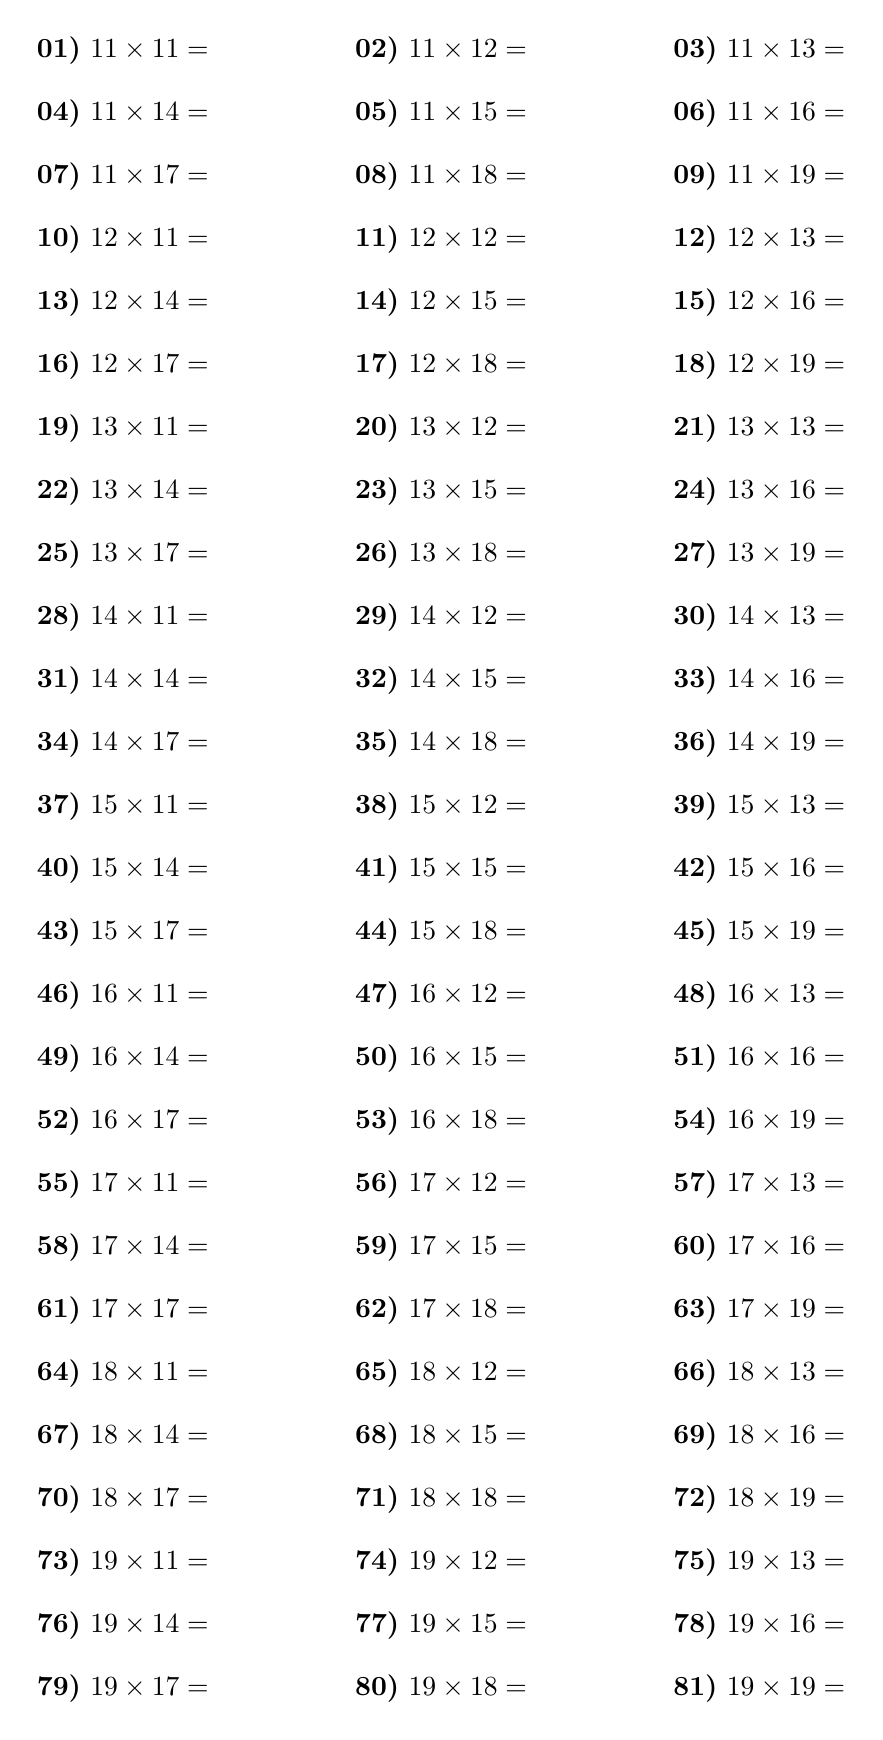
\begin{tikzpicture}
		\foreach \x in {11,...,19}
		\foreach \y in {11,...,19}
			{
				\stepcounter{total}
				\node at (\value{xcord} * \textwidth / 3, -\value{ycord}*0.8) {\textbf{\ifnum\value{total}<10
				0\fi\thetotal)} $\x \times \y =$};
		\stepcounter{xcord}		\ifnum\value{xcord}=3
		\setcounter{xcord}{0}
		\stepcounter{ycord}
		\fi
		}
	\end{tikzpicture}

\end{center}

\section{速算及巧算}
\subsection{计算总和}
\begin{enumerate}
	\item $1-2+3-4+5-6+7-8+9-10+11=$

	\item $3+5+7+9+11+13+15+17+19+21=$

	\item $100-99+98-97+96-95+94-93+93-92+91=$

	\item $6+8+10+12+14+16+18+20+22+24=$

	\item $1 + 2 + 3 + \ldots + 100 = $

	\item $2 + 4 +6 + \ldots + 100 = $

	\item $1 + 3 + 5 + \ldots + 99 = $

	\item $5 + 10 + 15 + \ldots + 100 = $

	\item $1 - (1+2) + (1+2+3) - (1+2+3+4) + \ldots - (1+2+\ldots+98) + (1+2+\ldots+99) = $

	\item $1-2+3-4+\ldots+2023-2024+2025=$

	\item $19+28+37+46+55+64+73+82+91+ \underline{\hspace{1cm}}=550$

	\item $2000-180+220-180+220-180+220-180+220-180+220=$

	\item $352.46-35.58-65.93-76.07-24.42=$

	\item $1+2+4+8+16+32+64+128+256+512+1024=$

	\item $8+89+899+8999+89999=$

	\item $8+88+888+8888+88888=$

	\item $28+208+2008+20008=$

	\item $24+63+52+17+49+81+74+38+95=$

	\item $1999.9+199.9+19.9+1.9=$

	\item $(7+9+11+13+\ldots+37)-(9+11+13+15+\ldots+35)=$

\end{enumerate}

\pagebreak
\section{速算和巧算2}

\begin{enumerate}

	\item $(6+8+10+12+\ldots+36)-(8+10+12+14+\ldots+34)=$

	\item $(1+4+7+10+\ldots+40)-(4+7+10+13+\ldots+37)=$
\end{enumerate}

\end{document}
